\documentclass[rgb,listoffigures,listoftables,final]{cam-thesis}

% Packages go here
\usepackage[acronym]{glossaries}
\usepackage{nomencl}
\usepackage{indentfirst}
\usepackage{bbm}
\usepackage{float}
\usepackage{graphicx}
\usepackage{longtable}

\makenomenclature
\makeglossaries

% Document Details
\title{Soccer Match Prediction}
\author{Group 3 - Bardia Parmoun \& Christopher Semaan}
\date{April 2025}

\degree{SYSC 5108: Deep Learning}
\program{MASc Electrical and Computer Engineering}
\college{Carleton University}

\location{Ottawa, Ontario}
\submissiondate{April 2025}

% PDF meta-info:
\subjectline{\@title}
\keywords{keyword 1, keyword 2, etc.}

\abstract{%
    Soccer is among the most popular sports around the world, and soccer matches attract millions of fans annually. This popularity has led to the growth sports betting market. Sports betting, especially on a complex game like soccer, comes with its own set of challenges due to the numerous known and unknown factors. As a result, it is a very good use case for the application of various machine learning techniques. This paper explores the use of deep learning, more specifically a multi-layered Feedforward Neural Network (\gls{fnn}), to predict the outcome of soccer matches. The model is able to predict home wins, away wins, and draws using a variety of historical and predictive features. The performance of the model was also compared with the pre-match odds of each game and it was concluded that the model performs almost as accurately as the professional odds-makers. With an accuracy that outperforms random choice by $15\%$, this paper showcases promising results for the use of machine learning in the realm of sports betting.
}

\acknowledgements{%
    The authors of this paper would like to express their sincere gratitude to Dr. Changcheng Huang for his great efforts, guidance, expert knowledge, and warm support throughout the semester. 
}

\newcommand{\mainmatter}{
    \pagenumbering{arabic}
    \setcounter{page}{1}
}

\begin{document}

\frontmatter
\pagenumbering{roman}

\mainmatter

\newacronym{xG}{xG}{Expected Goals}
\newacronym{svm}{SVM}{Support Vector Machines}
\newacronym{knn}{KNN}{K-Nearest Neighbours}
\newacronym{fnn}{FNN}{Feedforward Neural Network}
\newacronym{cnn}{CNN}{Convolutional Neural Network}
\newacronym{rnn}{RNN}{Recurrent Neural Network}
\newacronym{lstm}{LSTM}{Long Short-Term Memory}

\nomenclature{$\pi(x)$}{Expected profit for betting on an individual outcome x}
\nomenclature{$O_x$}{The odds for outcome x}
\nomenclature{$\mathbbm{1}_x$}{Indicator function for whether outcome x occurred or not}
\nomenclature{$\pi(X)$}{Expected profit for betting on a set of outcomes (X)}

% Input Chapters:
\chapter{Introduction}
    \section{Motivation}
    Soccer is already the most popular sport in the world, but it is still growing. The most watched soccer league in the world, the Premier League, is watched in 900 million homes worldwide, but it has seen further growth in new markets such as the United States \cite{premwatchcount}. Last season, in the United States, the Premier League beat their average viewer record by 4\% from the previous year, and their single match viewer count record reached 2.12 million \cite{uswatchcount}. Along with the growth in viewership, a significant growth in the visibility of gambling and sports betting has been observed. This season, 11 out of the 20 Premier League clubs have a gambling company as their main shirt sponsor compared to four clubs 10 years ago \cite{shirtsponsor}. The shirt sponsor is the most prominent on each shirt, so viewers will be sure to notice this prevalence. With sports betting estimated to grow 10.8\% from 2023 to 2030, more and more people are using sports betting as a way to make money or get engaged with sports \cite{sportsbettingmarket}. 

    \section{Objective}
    The objective of predicting match results is to see if it is feasible to profit from gambling using deep learning models. With unassisted betting, there is always the factor of emotional connection and perceived bias towards the teams or players involved. In some cases, the human factor in the sport can be a positive, but predictive modeling can be more consistent and use statistics to back it up. Additionally, to encourage more bets and participation, most odd makers tend to make bets in favour of wins as opposed to draws. A model that can be more accurate than a human could be a useful tool in making sports betting less risky.

    \section{Why Deep Learning?}
    Deep learning makes sense to predict soccer matches since the goal is to model nonlinear relationships from a large data set with many parameters. Traditional models might struggle to capture the complex interactions between variables such as team match performance and historical performance. Deep learning is much better at identifying hidden patterns and correlations within high-dimensional data. With the unpredictability of soccer, a deep learning model can be more robust in handling infrequent data points. The best example of this in any sport is when the performance parameters of the match may suggest a winner, but the result is an upset. Deep learning models can also continue to learn through the use of online learning if more data is available and adapt to additional data and trends.

    \section{Dataset Requirements}
    To be able to measure the success of a sports betting model, the model will require pre-match data. For most betting platforms, bets are placed before the match starts, so the dataset requires data that can be collected solely before the match. Predictive match statistics would also fit this requirement as long as they can be collected before the match. The data set will also require real data on the odds of betting for each match to be able to measure the profitability and performance of the model.
    
\chapter{Background}
    The problem of predicting the result of a soccer match is quite complex due to the unpredictable and variable nature of the sport. Due to this complexity, this problem has not been fully solved to a reliably high level of accuracy. This level of unpredictability has made this sport quite popular for betting which has also resulted in a lot of efforts in odds making.
    
    \section{Odds Making}
    In sports, odds indicate the likelihood of a specific outcome. In the case of soccer, there are only 3 possible outcomes: home team winning, away team winning, or a draw. Odds are the ratio of the amount of money that a person can earn from their original bet. For example, betting on an outcome with the odds of $5:1$ means that one can earn 5 dollars for every dollar that they bet if the outcome happens. By definition, odds are inversely correlated with the probability of that outcome happening. In other words, the higher the odds, the less probable that outcome is \cite{investopedia}. From this, the expected profit ($\pi$) for betting on outcome ($x$) with odds ($O$), is calculated as follows:
    \[
        \pi(x) = O_x \cdot \mathbbm{1}_x  - 1
    \]
    
    This formula shows that the potential profit of betting on an outcome $x$ is simply the potential earned money from the odds of that outcome minus the original betting amount. As such, the net profit of betting on $n$ soccer matches with outcomes $X = x_1, x_2, ..., x_n$ is defined as follows:
    \[
        \pi_{net} = \pi(X) = \sum_{i=1}^n \pi(x_i) = \sum_{i=1}^n \left[O_{x_i} \cdot \mathbbm{1}_{x_i} - 1\right]
    \]

    It is worth noting that for a model that aims to predict the most likely outcome, this metric will usually be a small number (or even a negative number) since the odds makers usually set the odds for the most likely outcome much lower than the unlikely outcomes. This results in the metric having greater penalties for incorrect guesses.  

    \section{Possible Solutions}
    Various approaches can be considered when designing a system that can predict soccer matches. The traditional method for predicting soccer matches involves the use of professional odds-makers. These are people who have great knowledge and often insider information about the game. Many businesses exist around this profession, such as \href{https://www.bet365.com/hub/en-gb/football}{Bet365}, \href{https://sportsbook.fanduel.com/soccer}{FanDuel}, etc. Another approach is the use of simpler machine learning techniques such as \gls{svm}, \gls{knn}, random forests, and linear regressions. Although these methods are easy to implement, they often fail to capture complex relations. Finally, as mentioned previously, deep learning methods can also be used. \gls{fnn} seems like a good candidate. The existence of historical features and their sequential nature suggest that \gls{rnn}, \gls{lstm} networks, and even \gls{cnn} can also be used.
    
    \section{A Survey of Existing Solutions}
    \subsection{Traditional Odds Making}
    Although traditional odds making seems to be the most common method, it tends to have its own biases and limitations, resulting in an accuracy of around $\sim 55\%$ at best \cite{socceranalytics}. Additionally, since odds-makers do not directly profit from the accuracy of their predictions, they tend to focus on the popularity of their bets instead. This means they usually try to make better odds for the fan-favourite outcomes (for example, a home win for the popular team) as opposed to draws due to their uninteresting nature.

    \subsection{Voting: FNN \& Random Forest}
    This approach involves the use of a voting model that picks the best result between an FNN model and a random forest model. The paper considers a variety of different features, such as match season, league name, home team name, away team name, and goal difference. The paper also considered 216743 soccer matches in 52 soccer leagues and 18 seasons. They also considered different weight strategies to help increase the presence of draws. The maximum accuracy achieved by this model was $\sim 46.6\%$ \cite{votingmodelexample}.

    \subsection{Sequential: RNN \& LSTM}
    This paper explored the use of sequential models by comparing the performance of RNN and LSTM networks. The dataset used by this paper included a variety of sequential features, such as goals scored by both teams, goal differences for both teams, point difference for the teams, results of the last 4 games won by each team, win streaks of each team with both 3 and 5 games, and finally loss streaks of each team with both 3 and 5 games. The dataset for this model contained matches from 2010-11 and 2017-18 of the English Premier League. It is worth noting that this model did not consider draws, and it was only able to predict wins and losses. The best performance achieved by this model was $\sim 81.75\%$ \cite{sequentialmodelexample}.

    \subsection{Random Forest with Gradient Boosting}
    This approach involves the use of more traditional machine learning approaches, such as decision trees and random forests. In this paper, a variety of features are considered, such as goal differences, rank differences, and goals per rank differences. The model was trained on 44341 international matches from 1872 to 2023, and it achieved an overall accuracy of $\sim 71.72\%$ \cite{randomforestexample}.
    
    \subsection{Multi-layered FNN}
    This approach involves the use of a multi-layer FNN. Similar to the previous models, it utilizes a variety of features, most importantly, includes team shots, shots on target, corners, fouls committed, yellow \& red cards, goals scored and conceded in the first half, and total goals scored and conceded. The model analyzes these features for the last 35 matches of the team. The model was trained on the last 350 Premier League matches and achieved an accuracy of $\sim 61.15\%$ \cite{fnnexample}.

    \subsection{Stacking: CNN, SVM, Regression, \& Random Forest}
    This model is the most complex approach when it comes to solving the problem. It is a stacking approach involving a wide range of machine learning techniques, including CNN, SVM, logistic regression, and random forest. This paper considers a wide range of features such as match date, home and away team, time of kick-off, game result, half-time goals, yellow \& red cards, temperature, relative humidity, participation, wind direction and speed, and weather conditions. For this paper, the English Premier League matches from 2019 to 2022 were considered. The accuracies of each model, in addition to the final stacked performance of the model, were calculated. The maximum accuracy reported by the model is $\sim 62.6\%$  \cite{stackingmodelexample}.
    
    \section{The Chosen Approach}
    For this project, a 5-layer FNN has been chosen. The main reason for this decision is the fact that it has been used in a variety of existing solutions. In addition, since all the dataset columns are simple numerical values, there is no need for complex mathematical operations such as convolutions, which eliminates the need for CNNs. Additionally, since the historical columns of the data have already been aggregated, there is no need for complex models such as RNN and LSTM networks. Furthermore, due to the complex nature of the problem, deep learning methods like FNNs are preferred over random forests.\\

    Since there are three possible outcomes for the problem, a model that performs randomly will have an average accuracy of $\frac{1}{3} \sim 33\%$. In addition, based on the papers that were previously discussed, the state-of-the-art solutions seem to have an average accuracy in the range of $\sim 40\%$ to $\sim 60\%$. As a result, this group aims to develop a model that has an accuracy of $\sim 50\%$.
    

\chapter{System Description}
    \section{Dataset Description}
    The size of the chosen dataset included 57,819 matches with 45 columns total \cite{kaggle}. The majority of columns included data about the form of the team across the whole season or the last four or six matches. There are also two predictive columns for \gls{xG}. Expected goals are the calculated metrics for the quality of chances created from shots taken by the team. There are also several columns related to betting odds and profit for the results of home win, draw, or away win. 
    \begin{center}
    \footnotesize
    \renewcommand{\arraystretch}{1.1}
    \begin{longtable}{ll}
        \caption{\normalsize Description of match dataset variables} \label{tab:match_variables} \\
        \hline
        Item & Description \\
        \hline
        \endfirsthead
    
        \hline
        Item & Description \\
        \hline
        \endhead
    
        \hline
        \endfoot
    
        \hline
        \endlastfoot
    
        id & Unique identifier for each match. \\
        team\_a\_mot\_x\_pos & Motivation of team A based on their position. \\
        team\_b\_mot\_x\_pos & Motivation of team B based on their position. \\
        team\_a\_ppg\_dif\_l4 & Points per game difference for team A in the last 4 matches. \\
        team\_a\_ppg\_dif\_l6 & Points per game difference for team A in the last 6 matches. \\
        team\_b\_ppg\_dif\_l4 & Points per game difference for team B in the last 4 matches. \\
        team\_b\_ppg\_dif\_l6 & Points per game difference for team B in the last 6 matches. \\
        team\_a\_ratio\_shotsOnTarget\_overall & Overall ratio of shots on target for team A. \\
        team\_a\_ratio\_shotsOnTarget\_l4 & Ratio of shots on target for team A in the last 4 matches. \\
        team\_a\_ratio\_shotsOnTarget\_l6 & Ratio of shots on target for team A in the last 6 matches. \\
        team\_b\_ratio\_shotsOnTarget\_overall & Overall ratio of shots on target for team B. \\
        team\_b\_ratio\_shotsOnTarget\_l4 & Ratio of shots on target for team B in the last 4 matches. \\
        team\_b\_ratio\_shotsOnTarget\_l6 & Ratio of shots on target for team B in the last 6 matches. \\
        odds\_ft\_1 & Betting odds for a home win. \\
        odds\_ft\_x & Betting odds for a draw. \\
        odds\_ft\_2 & Betting odds for an away win. \\
        predict\_xg\_overall\_team\_a & Predicted total expected goals for team A. \\
        predict\_xg\_overall\_team\_b & Predicted total expected goals for team B. \\
        predict\_xg\_home\_team\_a & Predicted expected goals for team A at home. \\
        predict\_xg\_away\_team\_b & Predicted expected goals for team B away. \\
        team\_a\_xg\_last4\_prematch & Expected goals for team A in the last 4 matches. \\
        team\_b\_xg\_last4\_prematch & Expected goals for team B in the last 4 matches. \\
        team\_a\_xga\_last4\_prematch & Expected goals against for team A in the last 4 matches. \\
        team\_b\_xga\_last4\_prematch & Expected goals against for team B in the last 4 matches. \\
        position\_a\_prematch & League position of team A before the match. \\
        position\_b\_prematch & League position of team B before the match. \\
        HomeWin & Binary indicator (1 or 0) if the home team won. \\
        Draw & Binary indicator (1 or 0) if the match was a draw. \\
        AwayWin & Binary indicator (1 or 0) if the away team won. \\
        division & Division or league in which the match is played. \\
        team\_a\_shots\_average & Average shots per match for team A. \\
        team\_b\_shots\_average & Average shots per match for team B. \\
        team\_a\_shots\_average\_l4 & Average shots per match in the last 4 matches for team A. \\
        team\_b\_shots\_average\_l4 & Average shots per match in the last 4 matches for team B. \\
        team\_a\_shots\_average\_l6 & Average shots per match in the last 6 matches for team A. \\
        team\_b\_shots\_average\_l6 & Average shots per match in the last 6 matches for team B. \\
        team\_a\_shots\_overall\_TSR & Total Shooting Ratio for team A. \\
        team\_b\_shots\_overall\_TSR & Total Shooting Ratio for team B. \\
        team\_a\_shots\_overall\_l4\_TSR & Total Shooting Ratio in the last 4 matches for team A. \\
        team\_b\_shots\_overall\_l4\_TSR & Total Shooting Ratio in the last 4 matches for team B. \\
        team\_a\_shots\_overall\_l6\_TSR & Total Shooting Ratio in the last 6 matches for team A. \\
        team\_b\_shots\_overall\_l6\_TSR & Total Shooting Ratio in the last 6 matches for team B. \\
        profit\_1 & Theoretical profit for betting on a home win. \\
        profit\_x & Theoretical profit for betting on a draw. \\
        profit\_2 & Theoretical profit for betting on an away win. \\
    \end{longtable}
    \end{center}

\section{Dataset Analysis}
    In order to detect the important features, a detailed correlation map of the dataset columns was prepared as follows:
    \begin{figure}[H]
        \centering
        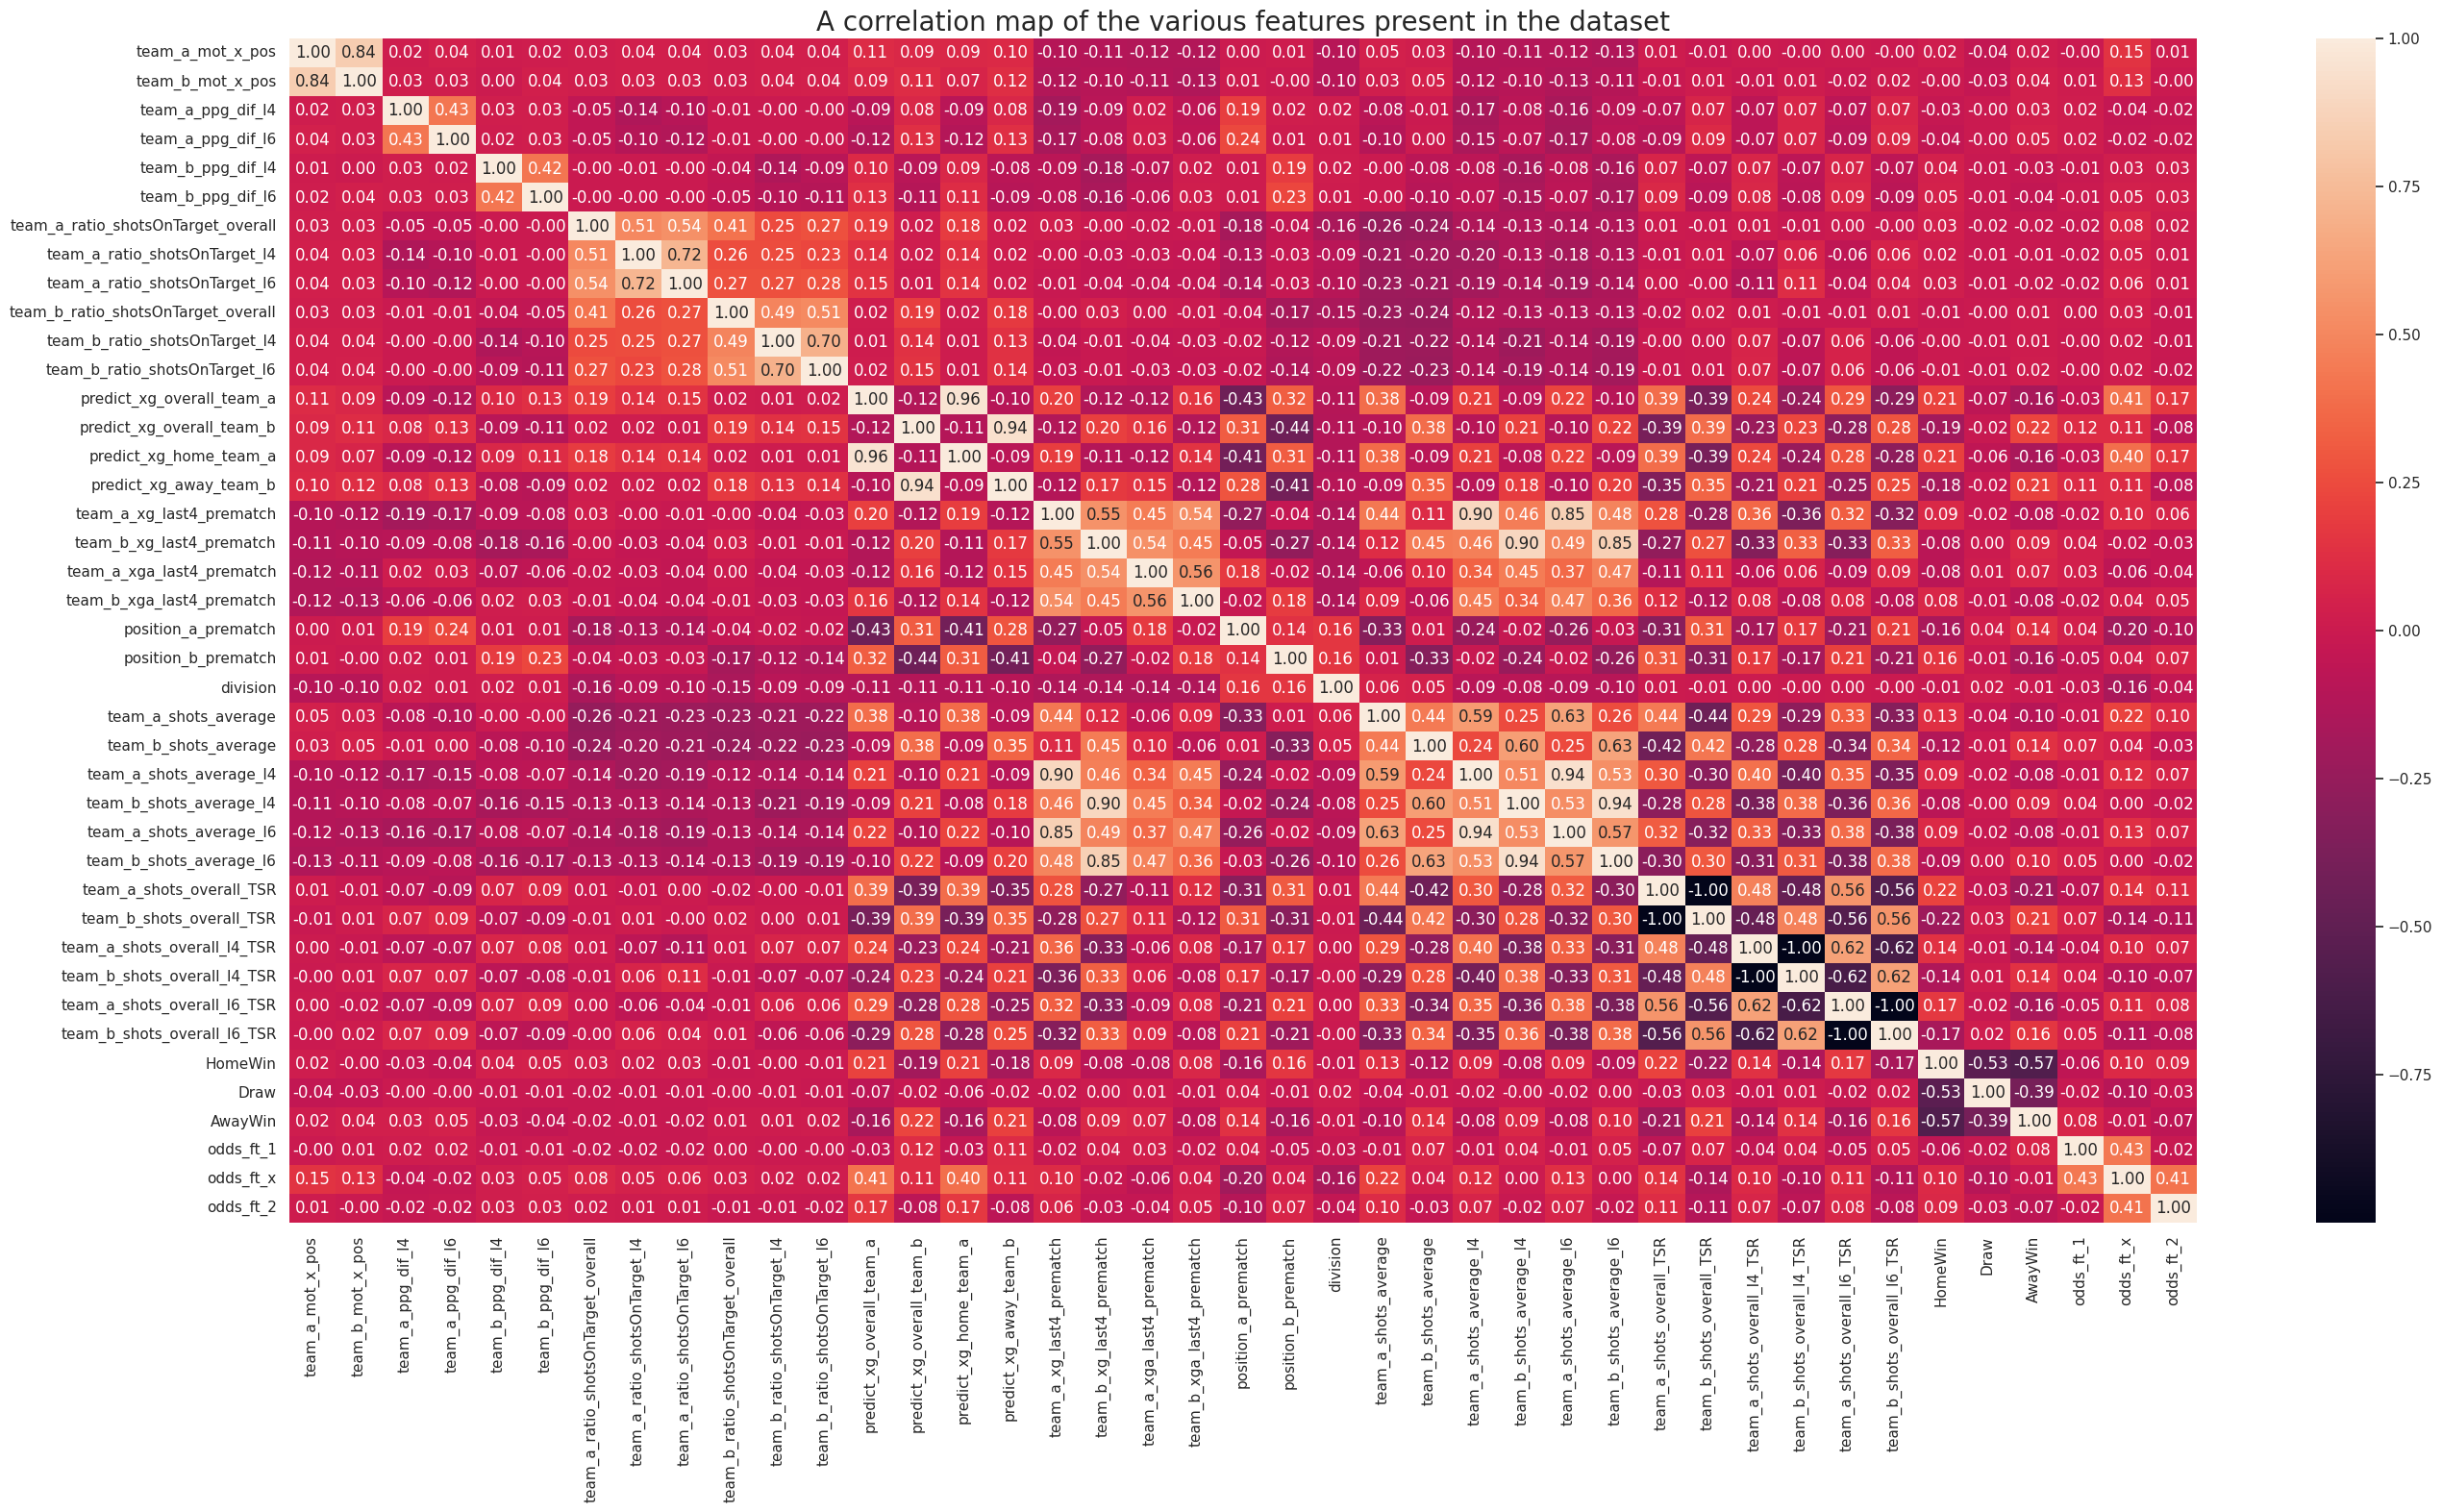
\includegraphics[width=\textwidth]{figures/correlationmap.png}
        \caption{Correlation map of all the columns}
        \label{fig:correlation-map}
    \end{figure}

    As shown in figure \ref{fig:correlation-map}, some features have non-negligible correlation with the match results features. A couple of these are the xG overall and the total shot ratio for both teams which are both above 0.2 correlation. Another important note is that draws have no direct correlation with any feature. The \texttt{Seaborn} library was used to generate the correlation map.\\
    
    Reflecting real soccer outcomes, this dataset had an imbalance in result count, with home wins being the most common occurrence. 
    \begin{figure}[H]
        \centering
        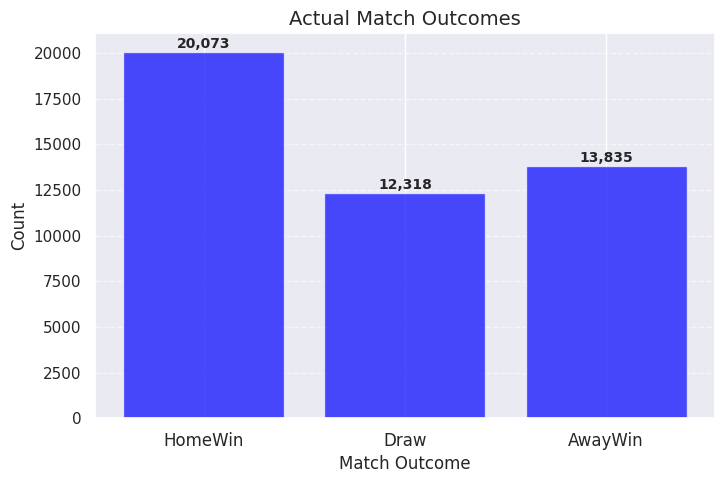
\includegraphics[width=0.7\textwidth]{figures/matchoutcomes.png}
        \caption{Chart showing total count of match results from the original dataset}
        \label{fig:matchoutcomes}
    \end{figure}

    As shown in figure \ref{fig:matchoutcomes}, the draw and away win counts are around 60\% and 65\% of the home win count. This is important to note, as there will be an unbalanced count if this data is directly used in training.
    
    \section{Data Pre-processing}
    The cleaning process first involved choosing columns deemed unnecessary for the model. The profit columns were not necessary as the model will be calculating profit using the equation mentioned in the Odds Making section (2.1). Any rows with empty data were also dropped. The dataset was also shuffled before any training was done to avoid any grouping in the order of the dataset. The odds columns were also ignored as they were used to compare the final performance of the model. Additionally, some columns were proven redundant since they were closely correlated with other columns. Specifically, 'team\_a\_ratio\_shotsOnTarget\_l6' and 'team\_a\_ratio\_shotsOnTarget\_l4' were highly correlated with other shooting metrics, and since an overall season parameter for shots on target was already included, the last 6 and last 4 match values were deemed redundant. Finally, the dataset was given an initial common 80/20 train/test split for the blind test data. The \texttt{Pandas} library was used to clean the dataset.

    
    \section{Model Description and Tools Used}
    As described in the Background section, the neural network was built from scratch using the \texttt{Tensorflow} library as a feedforward network with the following structure:

    \begin{figure}[H]
        \centering
        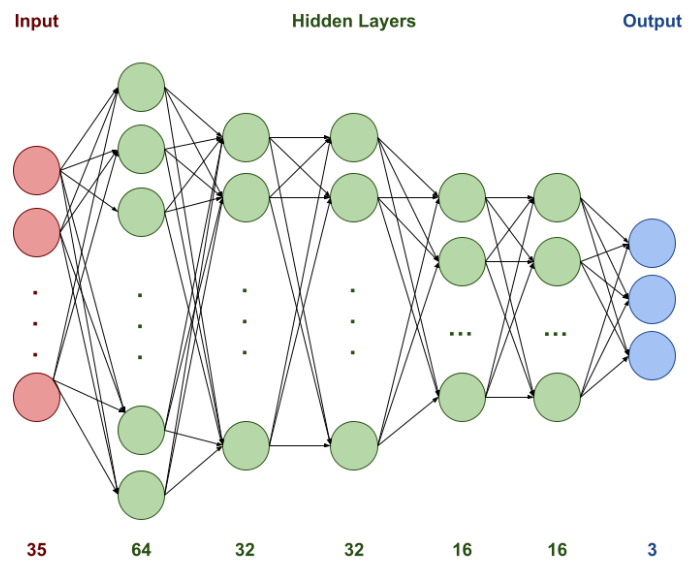
\includegraphics[width=0.7\textwidth]{figures/modelstructure.png}
        \caption{Diagram of the feedforward network structure}
        \label{fig:modelstructure}
    \end{figure}

    Here is a detailed description of the network:
    \begin{center}
    \renewcommand{\arraystretch}{1.2}
    \begin{longtable}{|l|c|r|}
      \caption{Neural network layer configuration}
      \label{tab:nn_layers} \\
      \hline
      \textbf{Layer (type)} & \textbf{Output Shape} & \textbf{Param \#} \\
      \hline
      \endfirsthead
    
      \hline
      \textbf{Layer (type)} & \textbf{Output Shape} & \textbf{Param \#} \\
      \hline
      \endhead
    
      \hline
      \endfoot
    
      \hline
      \endlastfoot
    
      dense (Dense) & (None, 64) & 2,048 \\
      batch\_normalization (BatchNormalization) & (None, 64) & 256 \\
      leaky\_re\_lu (LeakyReLU) & (None, 64) & 0 \\
      dropout (Dropout) & (None, 64) & 0 \\
      dense\_1 (Dense) & (None, 32) & 2,080 \\
      batch\_normalization\_1 (BatchNormalization) & (None, 32) & 128 \\
      leaky\_re\_lu\_1 (LeakyReLU) & (None, 32) & 0 \\
      dropout\_1 (Dropout) & (None, 32) & 0 \\
      dense\_2 (Dense) & (None, 32) & 1,056 \\
      batch\_normalization\_2 (BatchNormalization) & (None, 32) & 128 \\
      leaky\_re\_lu\_2 (LeakyReLU) & (None, 32) & 0 \\
      dropout\_2 (Dropout) & (None, 32) & 0 \\
      dense\_3 (Dense) & (None, 16) & 528 \\
      batch\_normalization\_3 (BatchNormalization) & (None, 16) & 64 \\
      leaky\_re\_lu\_3 (LeakyReLU) & (None, 16) & 0 \\
      dropout\_3 (Dropout) & (None, 16) & 0 \\
      dense\_4 (Dense) & (None, 16) & 272 \\
      batch\_normalization\_4 (BatchNormalization) & (None, 16) & 64 \\
      leaky\_re\_lu\_4 (LeakyReLU) & (None, 16) & 0 \\
      dropout\_4 (Dropout) & (None, 16) & 0 \\
      dense\_5 (Dense) & (None, 3) & 51 \\
    \end{longtable}
    \end{center}

    The final count of input parameters was 35 after cleaning. The model's layer sizes funnel down from 64 to 32 to 16 neurons, with the latter two having 2 consecutive layers. The output parameters are just the 3 possible match results, which are one-hot encoded. Each hidden layer had L2 regularization, batch normalization, leaky $ReLU$, and dropout applied, which can be seen in table \ref{tab:nn_layers}.\\

    Regularization was used at a 0.2 factor, which is relatively high, along with a dropout of 0.2 to solve overfitting issues. Batch normalization was also used to speed up training. Leaky $ReLU$ was applied to prevent dead neuron issues. An adaptive learning rate was used starting at 0.1 and applying a 3-epoch patience factor using the Adam optimizer. This ensures that the model can have an initial big jump in its learning, which slowly plateaus as the model converges.
    
    \section{Training \& Testing strategy}
    To ensure effective training and testing, $20\%$ of the dataset was reserved as a blind test set. The remaining $80\%$ was used to train the model through a two-stage approach: \\ 
    
    Initially, 5-fold cross-validation was applied to the training data, with each fold splitting the data further into $70\%$ training, $10\%$ validation, and $20\%$ testing. This allowed the model’s performance to be evaluated across a variety of data splits for greater reliability and allowed the team to calculate statistical measures such as mean and standard deviation. The final model was trained using a 90/10 train/validation split on the training data. In both stages, the model was trained for 50 epochs with a batch size of 32. Additionally, because it was discovered that home wins occurred far more frequently than draws or away wins, balanced class weights were used to prevent the model from favoring the majority class. This helped improve the model's ability to predict the other outcomes, particularly Draw and AwayWin.

    \section{Simple Odds Model}
    As previously mentioned, a simple model was developed using the existing odds to evaluate the performance of the FNN model. The odds model predicts the outcome with the smallest odds as the match outcome. In case of draws, the model favours home wins over the other two outcomes and away wins over draws to account for the class imbalance in the dataset. It is worth noting that this model was also run alongside the FNN model during both cross-validation and the blind test run.
    
    \section{Model Implementation}
    To implement this project, the group utilized \texttt{Python} and \texttt{Google Colab}. The team also used popular \texttt{Python} libraries, such as \texttt{TensorFlow} for model training; \texttt{NumPy}, \texttt{Pandas}, and \texttt{Scikit Learn} for data analysis; and \texttt{Seaborn}, and \texttt{Matplotlib} for data visualization. A \texttt{GitHub} repository containing the complete implementation of the project is located at: \url{https://github.com/bardia-p/soccer-match-predictor}.
    
    
\chapter{Numerical Results}
    \section{Existing Odds Performance on Training Data}
    As previously mentioned, the existing odds are used to evaluate the performance of the model. As a result, the accuracy of existing odds was initially evaluated on the entire training set (46226 soccer matches). The following confusion matrix was created by running the simple odds model on the training data:
    \begin{figure}[H]
        \centering
        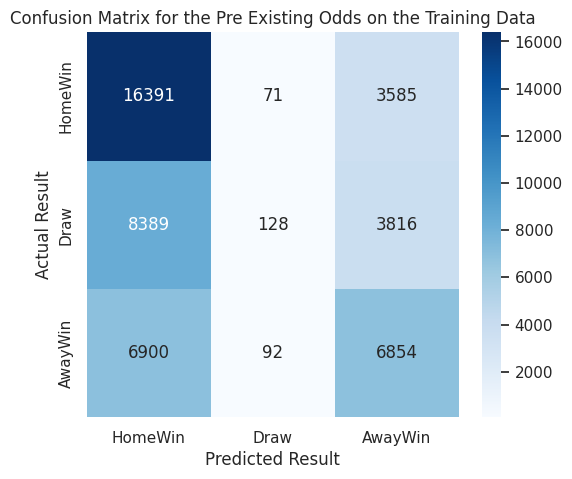
\includegraphics[width=0.55\textwidth]{figures/cm_existing_odds_training.png}
        \caption{Confusion matrix obtained from the odds on the training data}
        \label{fig:cm-odds-training}
    \end{figure}

    As shown in figure \ref{fig:cm-odds-training}, the existing odds only have an accuracy of $\sim 50.56\%$. This finding is in line with what was discussed in section 2.3.1. Additionally, it can be seen that the odds are heavily biased against draws since it was only able to predict 291 draws out of the 12318 draw matches. Furthermore, the profit metric described in 2.1 was run on the model, which resulted in a net profit of $\$-2401.6$. Although this value is low, as expected, the profit value came from spending $\$46226$.
    
    \section{Model Performance During Cross-Validation}
    As previously mentioned, the performance of the model was evaluated using 5-fold cross-validation. In addition, the simple odds model was run in parallel to the FNN model to obtain profit values. The results of this experiment are as follows:
    \begin{table}[h]
        \centering
        \caption{Performance metrics of both models during cross-validation}
        \vspace{1em}
        \label{tab:cross-validation-metrics}
        \begin{tabular}{lcc}
            \hline
            Metric                 & Mean      & Standard Deviation \\
            \hline
            F1 Score - FNN         & 46.28     & 1.28               \\
            Accuracy - FNN         & 46.43\%   & 2.23\%             \\
            Profit - FNN           & \$-441.47 & \$122.94           \\
            Profit - Odds Model    & \$-505.19 & \$40.79            \\
            \hline
        \end{tabular}
    \end{table}

    For this experiment, the model was only trained on 32358 soccer matches in each fold, which explains its slightly poorer performance. As shown in table \ref{tab:cross-validation-metrics}, the model performs slightly worse than the existing odds when it comes to accuracy; however, its accuracy value seems fairly consistent, as indicated by the standard deviation. Additionally, the low F1 score is mainly due to the poor recall of the model. This indicates that the model is quite strict with its predictions, resulting in a lot of false negatives. The profit metrics were calculated from the testing portion of the experiment or 9245 matches (20\% of the training data). In other words, these metrics should be read as the model earning that much amount for spending $\$9245$. In this experiment, it can be seen that the FNN Model slightly outperforms the Odds Model on average (by $\sim \$60$); however, it can also be seen that the FNN Model's standard deviation is much higher than the Odds Model's. Both of these results are because the FNN Model is less biased towards draws. In other words, the FNN Model is more willing to predict draws resulting in higher profits on average but also wider variations due to draws having very small gains in comparison to the other outcomes.
    
    \section{Final Model Training Performance}
    As previously mentioned, the final model was trained on the entire training dataset with a 90/10 training/validation split. The training process lasted for 50 epochs. The following diagram shows the performance of the model for each epoch:
    \begin{figure}[H]
        \centering
        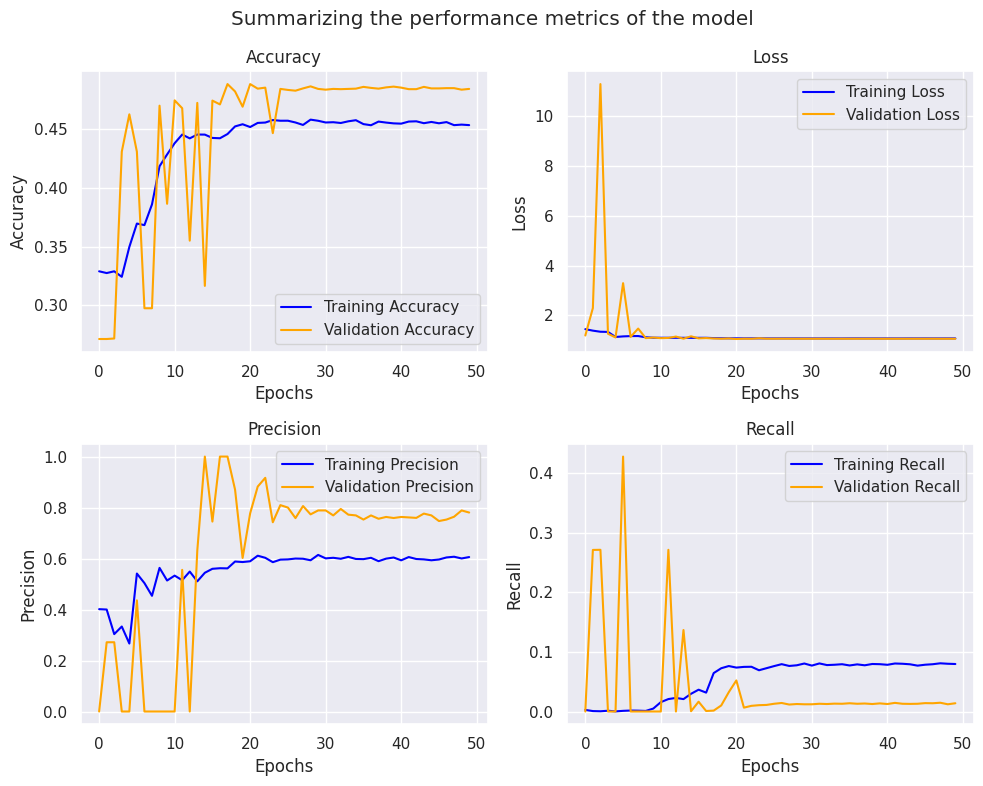
\includegraphics[width=0.95\textwidth]{figures/model_performance.png}
        \caption{A summary of the training performance of the final model}
        \label{fig:model-performance}
    \end{figure}

    As shown in figure \ref{fig:model-performance}, the model was able to achieve a maximum validation accuracy of $\sim 48.43\%$. In addition, it can be seen that the model has a really good validation of precision of around $\sim 78.05\%$ and a small validation loss of $1.05$. These indicate that the model is not overfit, and it is quite accurate in its positives; however, the validation recall is quite low at $\sim 1.38\%$, which indicates that the model is way too strict, resulting in a lot of false negatives. This can be an indicator of the model being underfit and needing more data.
    
    \section{Blind Test Performance}
    As previously mentioned, both the FNN and Odds models were evaluated on blind test data (11557 matches). The results are as follows:
    \begin{figure}[H]
        \centering
        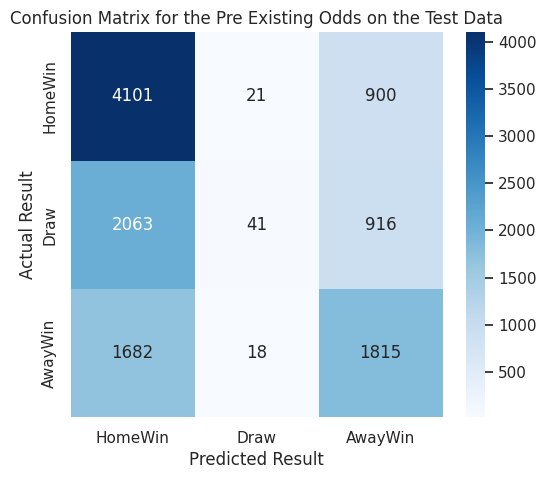
\includegraphics[width=0.55\textwidth]{figures/cm_existing_odds_testing.png}
        \caption{Confusion matrix obtained from the odds on the blind test data}
        \label{fig:cm-odds-testing}
    \end{figure}

    \begin{figure}[H]
        \centering
        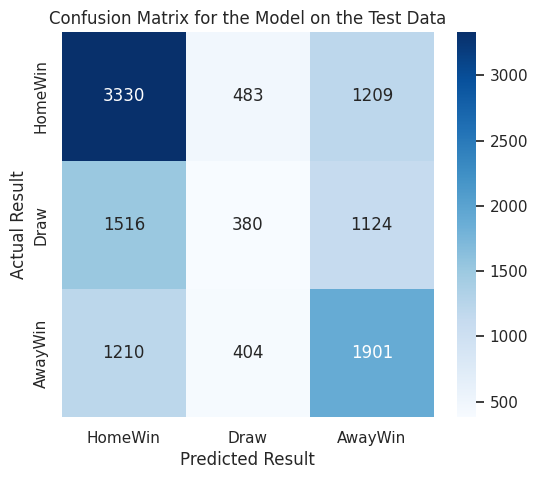
\includegraphics[width=0.55\textwidth]{figures/cm_model_testing.png}
        \caption{Confusion matrix obtained from the FNN on the blind test data}
        \label{fig:cm-odds-testing}
    \end{figure}

    The following metrics were also obtained:
    \begin{table}[h]
        \centering
        \caption{Performance metrics of both models on the blind test}
        \vspace{1em}
        \label{tab:blind-test-metrics}
        \begin{tabular}{lcc}
            \hline
            Metric                 & Value     \\
            \hline
            F1 Score - FNN         & 45.68     \\
            Accuracy - FNN         & 48.55\%   \\
            Accuracy - Odds Model  & 51.54\%   \\
            Profit - FNN           & \$-372.68 \\
            Profit - Odds Model    & \$-330.72 \\
            \hline
        \end{tabular}
    \end{table}

    As shown in table \ref{tab:blind-test-metrics}, the model's F1 score and accuracy were within the range that was predicted during cross-validation, which proves that it behaves quite consistently; however, it can be seen that the model slightly underperforms on the profit metric. Furthermore, it can be seen that the gap between the accuracies of the Odds Model and the FNN Model has increased. This further shows the inconsistencies of the odds. 
    
    \section{Findings}
    In summary, it can be seen that the FNN Model performs quite close to the existing odds. In addition, the accuracy of the FNN model ($\sim 48\%$) outperforms random by around $15\%$ and is very close to the initial prediction that the team made in section 2.4.\\

    It is worth noting that the FNN model was able to outperform the previously published voting model discussed in section 2.3.2, and it demonstrated similar performance to the traditional odds that were discussed in section 2.3.1. It can also be seen that the model did not perform as closely as the rest of start of the art models that were discussed in section 2.3, but the general structure of this FNN model is much simpler, and the features that were utilized by it are readily available.\\

    Finally, the team observed a hard limit $\sim 50\%$ on the maximum accuracy of the FNN model. This indicates that the model is probably underfit, which could be improved through the use of more training data and possibly even more features. Following the stacking model discussed in 2.3.6, this team recommends the incorporation of player information (e.g., ranking, age) and environmental factors (e.g., wind).

\chapter{Conclusion}
    This model's best statistical run reached an accuracy of 48.43\%, and it better predicted the frequency of Draws and Away Wins compared to traditional odds makers. This suggests the model captures certain patterns that odds makers may ignore when setting odds.\\
    
    To improve overall performance, future iterations could include more data samples from more matches, which could help improve learning. Another improvement would be the inclusion of player-specific features or more diverse team-related factors, such as passing or ball-possession-related statistics. These additions could help capture finer details about the match.\\
    
    This group learned that the sport is full of hidden variables that cannot always be captured by statistics. An example is a match between Manchester City and Cardiff City, where despite Manchester City holding 74\% possession, having 10 shots on target compared to Cardiff’s 4, and the odds for a Cardiff win were only 9:1, Cardiff still won 2–0 \cite{socceranalytics}. This illustrates that even with all the statistics favouring one team, the result is still hard to predict. 

% Bibliography
\bibliographystyle{unsrt}
\bibliography{bibliography}

\end{document}